\documentclass[12pt]{article}
\usepackage{latexsym,amssymb,amsmath} % for \Box, \mathbb, split, etc.
% \usepackage[]{showkeys} % shows label names
\usepackage{cite} % sorts citation numbers appropriately
\usepackage{path}
\usepackage{url}
\usepackage{verbatim}
\usepackage[pdftex]{graphicx}
\usepackage{color}

\usepackage{multicol}

% horizontal margins: 1.0 + 6.5 + 1.0 = 8.5
\setlength{\oddsidemargin}{0.0in}
\setlength{\textwidth}{6.5in}
% vertical margins: 1.0 + 9.0 + 1.0 = 11.0
\setlength{\topmargin}{0.0in}
\setlength{\headheight}{12pt}
\setlength{\headsep}{13pt}
\setlength{\textheight}{625pt}
\setlength{\footskip}{24pt}

\renewcommand{\textfraction}{0.10}
\renewcommand{\topfraction}{0.85}
\renewcommand{\bottomfraction}{0.85}
\renewcommand{\floatpagefraction}{0.90}

\makeatletter
\setlength{\arraycolsep}{2\p@} % make spaces around "=" in eqnarray smaller
\makeatother

% change equation, table, figure numbers to be counted inside a section:
\numberwithin{equation}{section}
\numberwithin{table}{section}
\numberwithin{figure}{section}

% begin of personal macros
\newcommand{\half}{{\textstyle \frac{1}{2}}}
\newcommand{\eps}{\varepsilon}
\newcommand{\myth}{\vartheta}
\newcommand{\myphi}{\varphi}

\newcommand{\IN}{\mathbb{N}}
\newcommand{\IZ}{\mathbb{Z}}
\newcommand{\IQ}{\mathbb{Q}}
\newcommand{\IR}{\mathbb{R}}
\newcommand{\IC}{\mathbb{C}}
\newcommand{\Real}[1]{\mathrm{Re}\left({#1}\right)}
\newcommand{\Imag}[1]{\mathrm{Im}\left({#1}\right)}

\newcommand{\norm}[2]{\|{#1}\|_{{}_{#2}}}
\newcommand{\abs}[1]{\left|{#1}\right|}
\newcommand{\ip}[2]{\left\langle {#1}, {#2} \right\rangle}
\newcommand{\der}[2]{\frac{\partial {#1}}{\partial {#2}}}
\newcommand{\dder}[2]{\frac{\partial^2 {#1}}{\partial {#2}^2}}

\newcommand{\nn}{\mathbf{n}}
\newcommand{\xx}{\mathbf{x}}
\newcommand{\uu}{\mathbf{u}}

\newcommand{\junk}[1]{{}}

% set two lengths for the includegraphics commands used to import the plots:
\newlength{\fwtwo} \setlength{\fwtwo}{0.45\textwidth}


\renewcommand{\labelitemi}{}
\renewcommand{\labelitemii}{}
\renewcommand{\labelitemiii}{}


% end of personal macros
% \input{inputFile.tex}


\begin{document}
\DeclareGraphicsExtensions{.jpg}



\begin{center}
\textbf{\Large AAAI Fellowship Application}\\[12pt] 
%\textbf{\Large } \\[6pt]
%\textbf{\Large } \\[6pt]
John Oberlin\\
Brown University, 2014\\
\end{center}

\section{Introduction}
%\cite{FooBar}

State of the art techniques in object detection and pose estimation
are powerful and general but usually run at a rate less than 1 Hz. Such a slow
rate makes it difficult to employ such techniques in real-time human-computer interaction.

Pitch the grocery video.

Our overall pipeline can be described as:

\begin{enumerate}
  \item Collect RGB-D data for objects.
  \item (Automatically) Train BoW model and kNN classifiers for objects.
  \item Use the classifiers and additional logic to provide 3D detections pose estimates of objects.
\end{enumerate}

Related work.

\section{Coordinating AI with Computer Vision}
MDPs, OO-MDPs, and POMDBs. How to create a perceptual system that plays well with planning.


\section{Teaching the System}
We call this process teaching and not training because it is an interaction used to collect
data not a program used to optimize a function.

\begin{figure}
  \begin{center}
    \begin{tabular}{l c}
      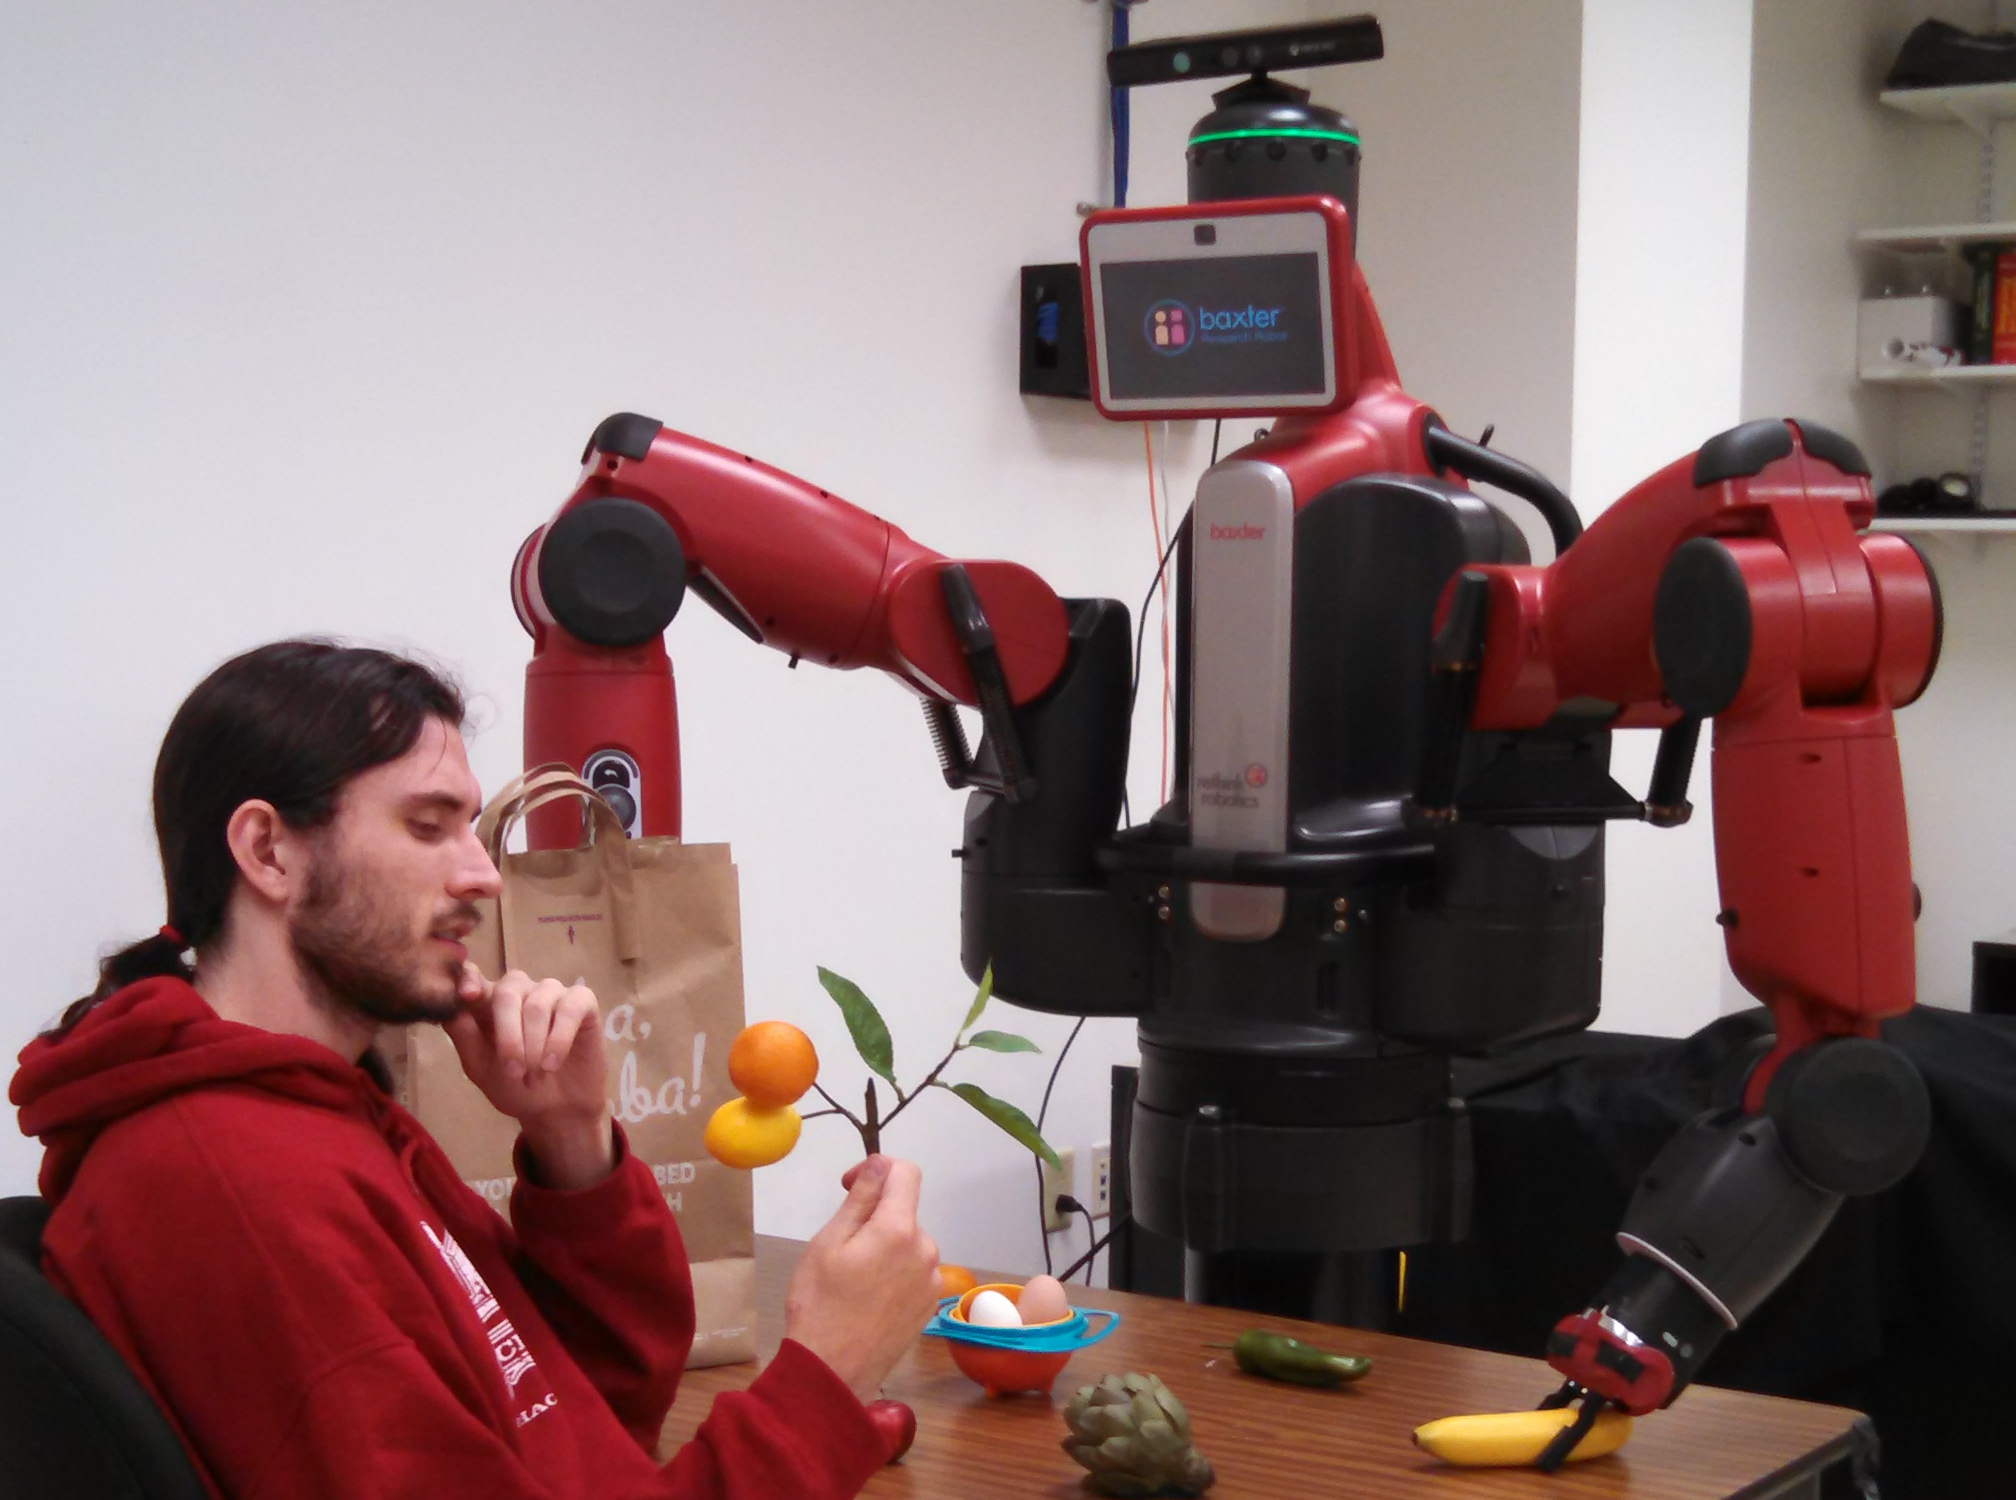
\includegraphics[width=200px, height=150px]{robo2.png} &
      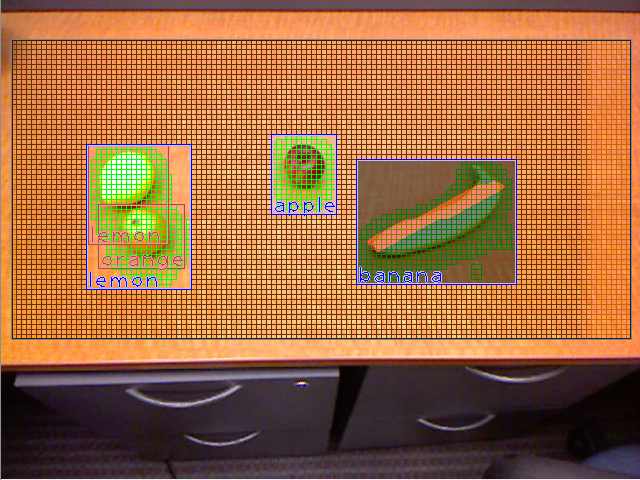
\includegraphics[width=200px, height=150px]{screen2.png} \\
    \end{tabular}
  \end{center}
  \caption{Teaching a robot to identify and manipulate objects can be as easy as bringing home
	    a bag of groceries.}
\end{figure}

\paragraph{Semi-Automatic Teaching}

\begin{enumerate}
  \item Repeat k times:
  \begin{enumerate}
    \item A human operator places the object in a robot's manipulator.
    \item The operator provides a base pose for the given grasp.
    \item The robot collects views of many different precisely known poses, together with models for self and background filtering.
  \end{enumerate}
\end{enumerate}

Where k might be around 3. 

Currently we train the system without a robot by manually adjusting the pose of the object and manually
annotating grasps. Eventually we would like to have fully automatic training, where the
robot grabs objects and coordinates base poses itself.


\section{Work Forecast}

\paragraph{Existing Software}
Manual training, robust pose estimation under good conditions.
Objectness
Fast Keypoints
SIFT descriptors
KMeans
BoW
Color Histogram
Depth Histogram
kNN
MDP

Green Boxes
Blue Boxes
Red Boxes

\paragraph{Current Directions}
Semi-automatic training
Automatic training
More geometric work

\paragraph{Broader Impact and Future Work}
working MDP's into the red box exploration and data collection so that we can interact with
large scale planners for tasks.


%\bibliographystyle{siam}
%\bibliography{proposal}

\newpage

\section{Attendance Statement}

  I have been paying attention to AI, Machine Learning, and Computer Vision since 2004. 
Regarding Computer Vision, I saw the progress of Neural Nets in the 90's swept under 
the rug by SIFT, HoG, and SVMs in the mid 2000's, only for neural nets to reclaim the throne in the 2010's.
At one time it was said that AI was "vision hard" and that solving Vision would
effectively solve AI. While that belief sweeps a bit under the rug, it is certainly true
that in the past Computer Vision has been a strong bottleneck in the development of AI and 
Robotics. 
  
  Recent advances in object detection on large data sets suggest that we are ready
to move beyond attacking vision in an isolated setting and begin integrating it in a
larger framework for planning in an interactive environment. I have training in state
of the art Computer Vision techniques and have been tracking the literature for a few
years now. 

  Work in Computer Vision has largely centered around hyperspecific problems concerning
single images. This focus has resulted in significant progress on such tasks, but the challenges of 
engineering real time systems has so far prevented interesting real world applications
or substantial spread of techniques to other communities. 

Two things have resulted from this dam in the flow of information. 
First, there are now many techniques in Computer Vision which are suited
to fast and effective partial solutions of problems such as object detection
but have been ignored in favor of much slower but slightly more effective state of the art
approaches.  Second, such techniques may be combined with the information available from
extra sensors and the ability of real time systems to capture additional images of the same scene
to form full solutions to multiple related problems (such as detection, segmentation, and pose estimation). 
 
I have seen already that combining elements of probabilistic planning and reasoning can boost
the performance of traditional Computer Vision and Machine Learning algorithms.  I want to
continue this approach to research, and attending AAAI will help me to fill in gaps in my
background that are necessary to carve out a career in multi-disciplinary AI.  
Planning and Markov Decision Processes are key elements that I want to master. Additionally,
I would like to explore topics such as Interactive Entertainment, Scheduling, Knowledge
Representation and Reasoning, and Reasoning Under Uncertainty in order to further my
understanding of Human-AI Interactions.

Finally, by attending AAAI I will be able to better understand the motivations, needs, and desires 
of AI and Robotics concentrators with regards to Computer Vision, which will enable me 
to complete my dissertation in a way that aligns with these communities' values.

\newpage

\section{Curriculum Vitae}
\textbf{\emph{Education}}\\
 \\
BS in Math, Florida State University, 2003-2006 \\
MA in Math, UC Berkeley, 2006-2008 \\
PhD program in Computer Science at U Chicago, 2010-2011 \\
PhD program in Computer Science at Brown University, 2011-Present \\
 \\ 
\textbf{\emph{Employment}}\\
\\
Developer Support Engineer, Havok, 2008-2009 \\
 \\
\textbf{\emph{Conference Papers}}\\
 \\
S. Naderi Parizi, J. Oberlin, P. Felzenszwalb.\\
\emph{Reconfigurable Models for Scene Recognition.}\\
IEEE Conference on Computer Vision and Pattern Recognition (CVPR), 2012\\
 \\
P. Felzenszwalb, J. Oberlin.  \\
\emph{Multiscale Fields of Patterns.}\\
To Appear, 2014 \\
 \\
\textbf{\emph{Conferences Attended}}\\
 \\
CVPR 2011\\
CVPR 2012 \\
 \\
\textbf{\emph{Teaching Experience}}\\
 \\
Being a TA in the UCB Math Deparment can be close to a full time teaching position, including
quiz design, office hours, and grading in addition to the intense recitation sections (which more closely resembled lectures). \\
\\
Calculus 1 TA\\
UC Berkeley, 2006-2007\\
Two sections in the Fall, three sections in the Spring, 30 students in each section, each section met with me
two or three times a week for a total of about three hours a week.\\
 \\
Linear Algebra and ODE TA\\
UC Berkeley, 2007-2008\\
Same configuration as calculus.\\
 \\
Algorithms Grad TA\\
Brown University, 2012-Present\\
\\
I am currently the Grad TA for the Algorithms class at Brown for the fourth semester. During this time the class has been
between 45 and 100 students each iteration.  I have been responsible for administering oral exams, holding office hours,
lots of grading (most of our problems are proof based), and managing a group of at least 6 Undergraduate TA's each semester.\\
 \\
\textbf{\emph{Departmental Service}}\\
 \\
Graduate Student Orientation Leader\\
Brown CS Department, Fall 2012\\
 \\
Computer Vision Reading Group Coordinator\\
Brown CS Department, 2012\\
 \\
Department Tea Organizer\\
Brown CS Department, 2012-Present\\
 \\
\textbf{\emph{Misc Research}}\\
 \\
Master's Thesis in Mathematics\\
UC Berkeley, Written 2006-2008\\
 \\
Research Experience for Undergraduates in Mathematics\\
Oregon State University, Summer 2005\\
 \\
Undergraduate Research Program in Physics\\
Florida State University, Summer 2004\\
 \\
Research Assistant in Molecular Biology\\
Florida State University, Summer 2003\\
 \\
\textbf{\emph{Hobbies}}\\
 \\
Gardening\\
Ballroom Dance\\
Martial Arts\\
Blacksmithing\\
3D Printing\\
 \\
\newpage

\section{Letter From Supervisor}

\newpage


\end{document}

